\begin{figure}[h!]
\centering
\begin{subfigure}[t]{.8\linewidth}
    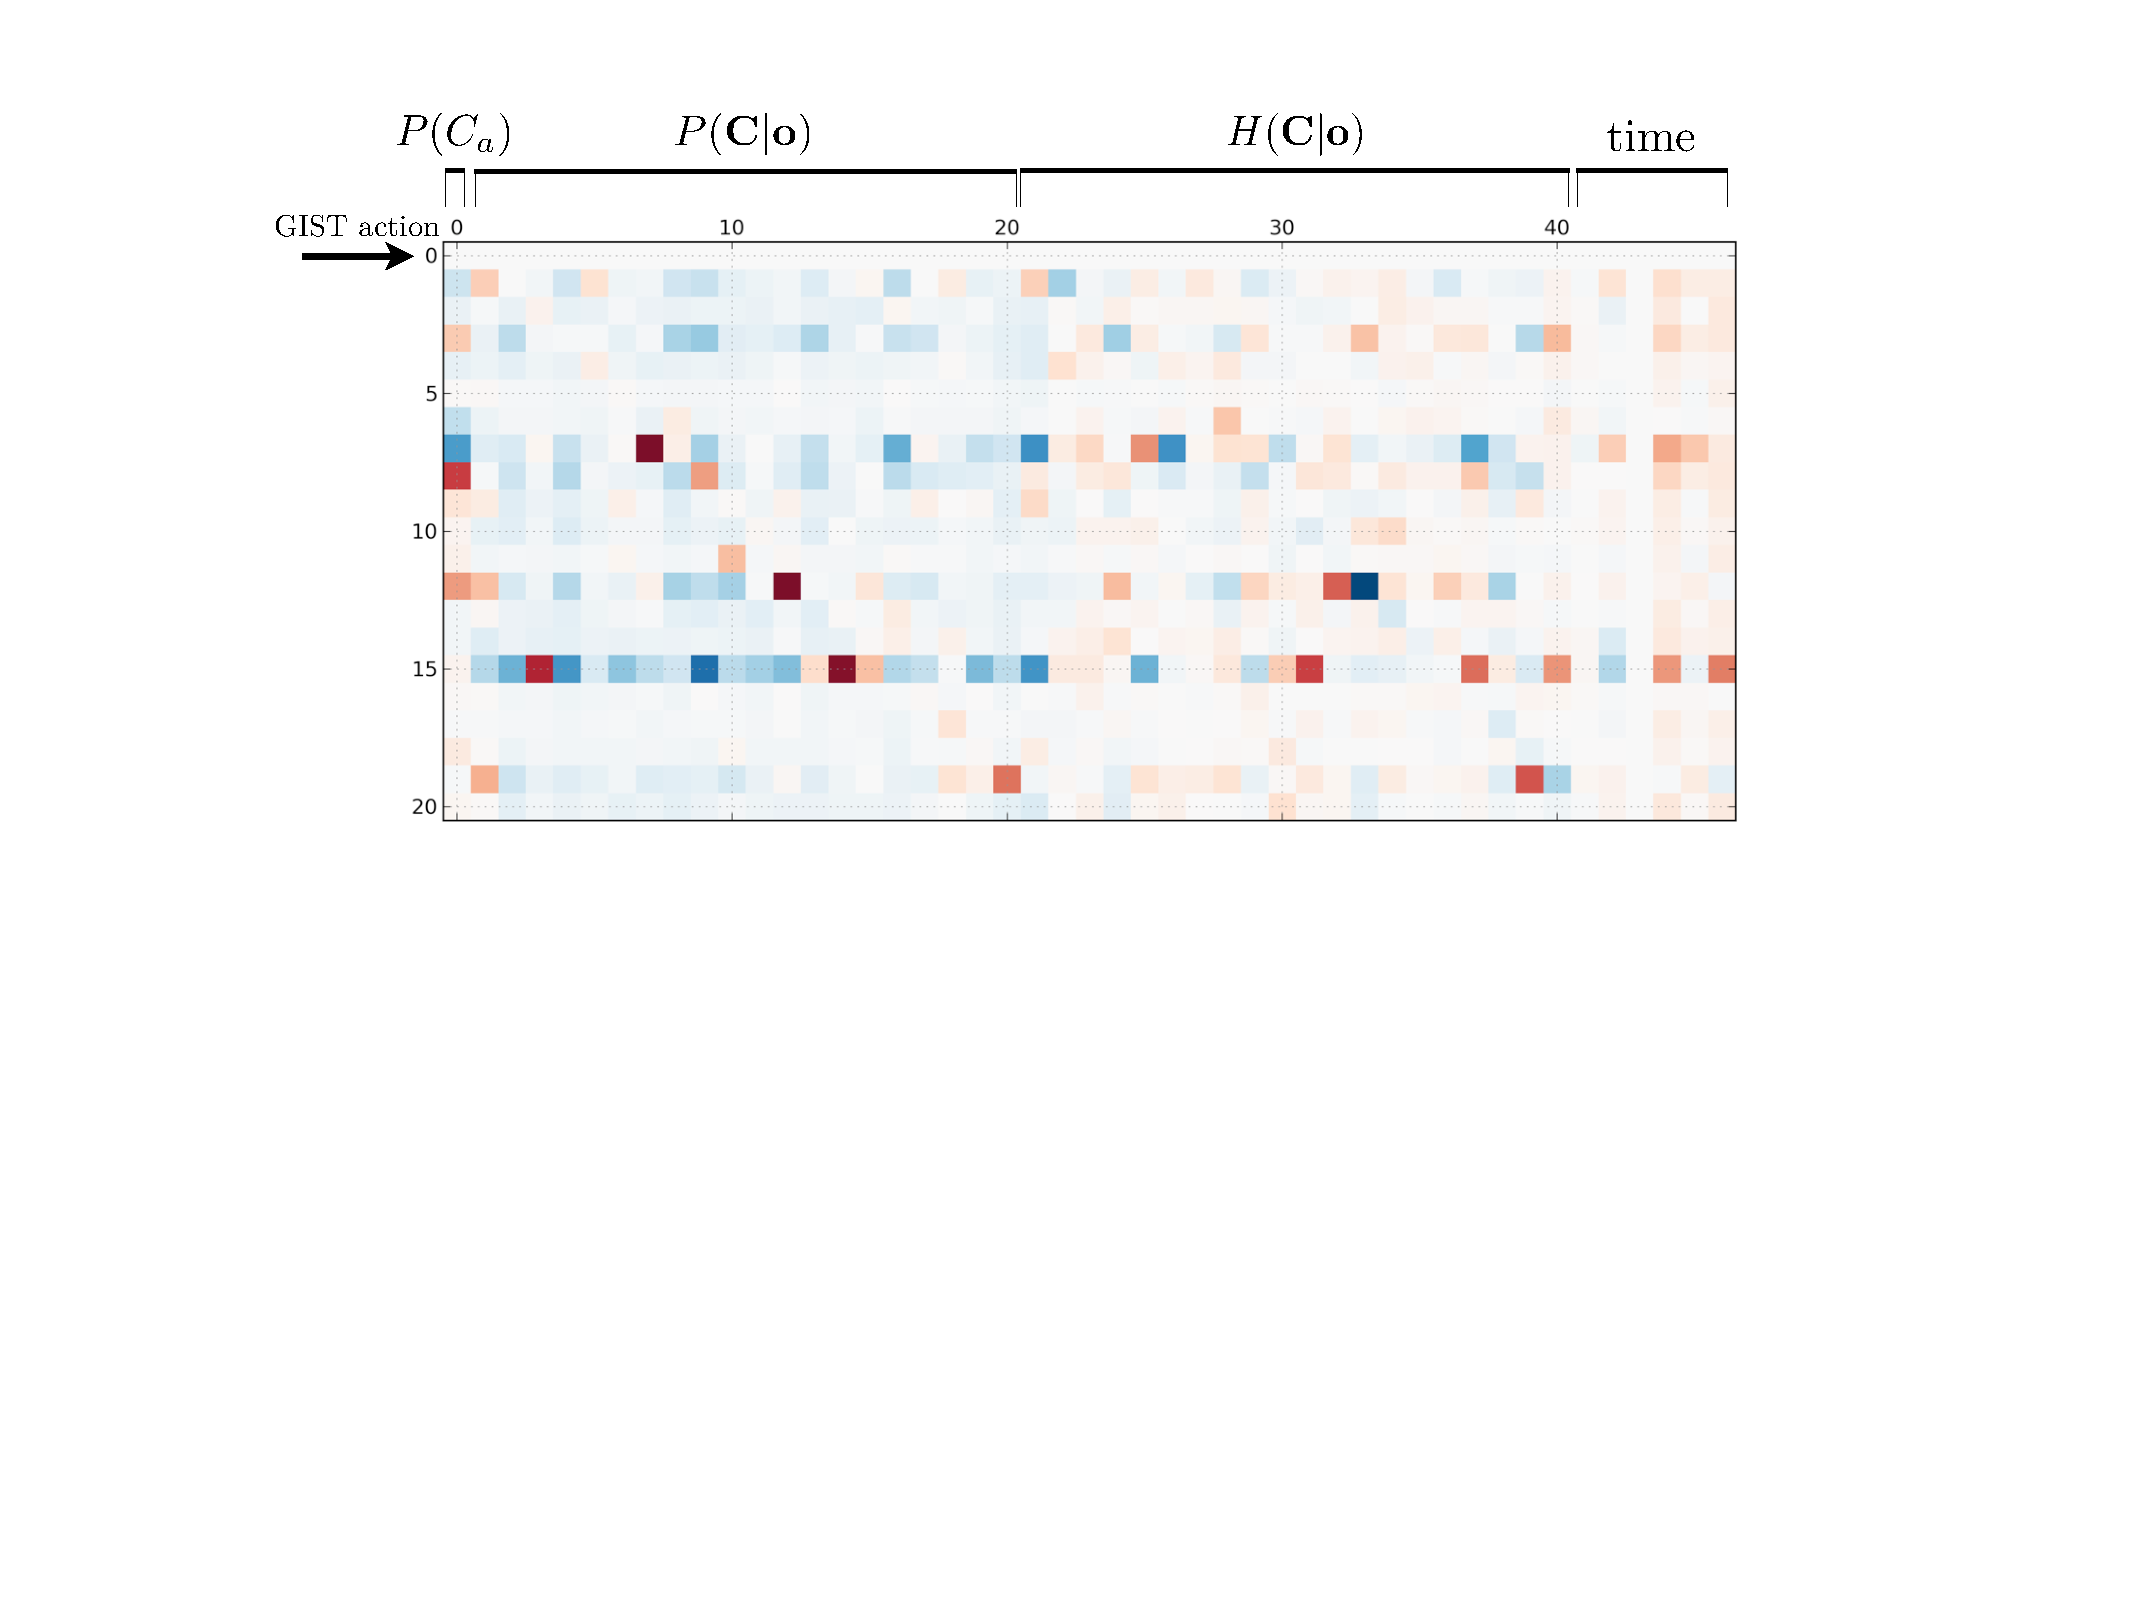
\includegraphics[width=\linewidth]{../../../2011-2012/figures/weights_greedy}
    \caption{Greedy}
\end{subfigure}\\
\begin{subfigure}[t]{.8\linewidth}
    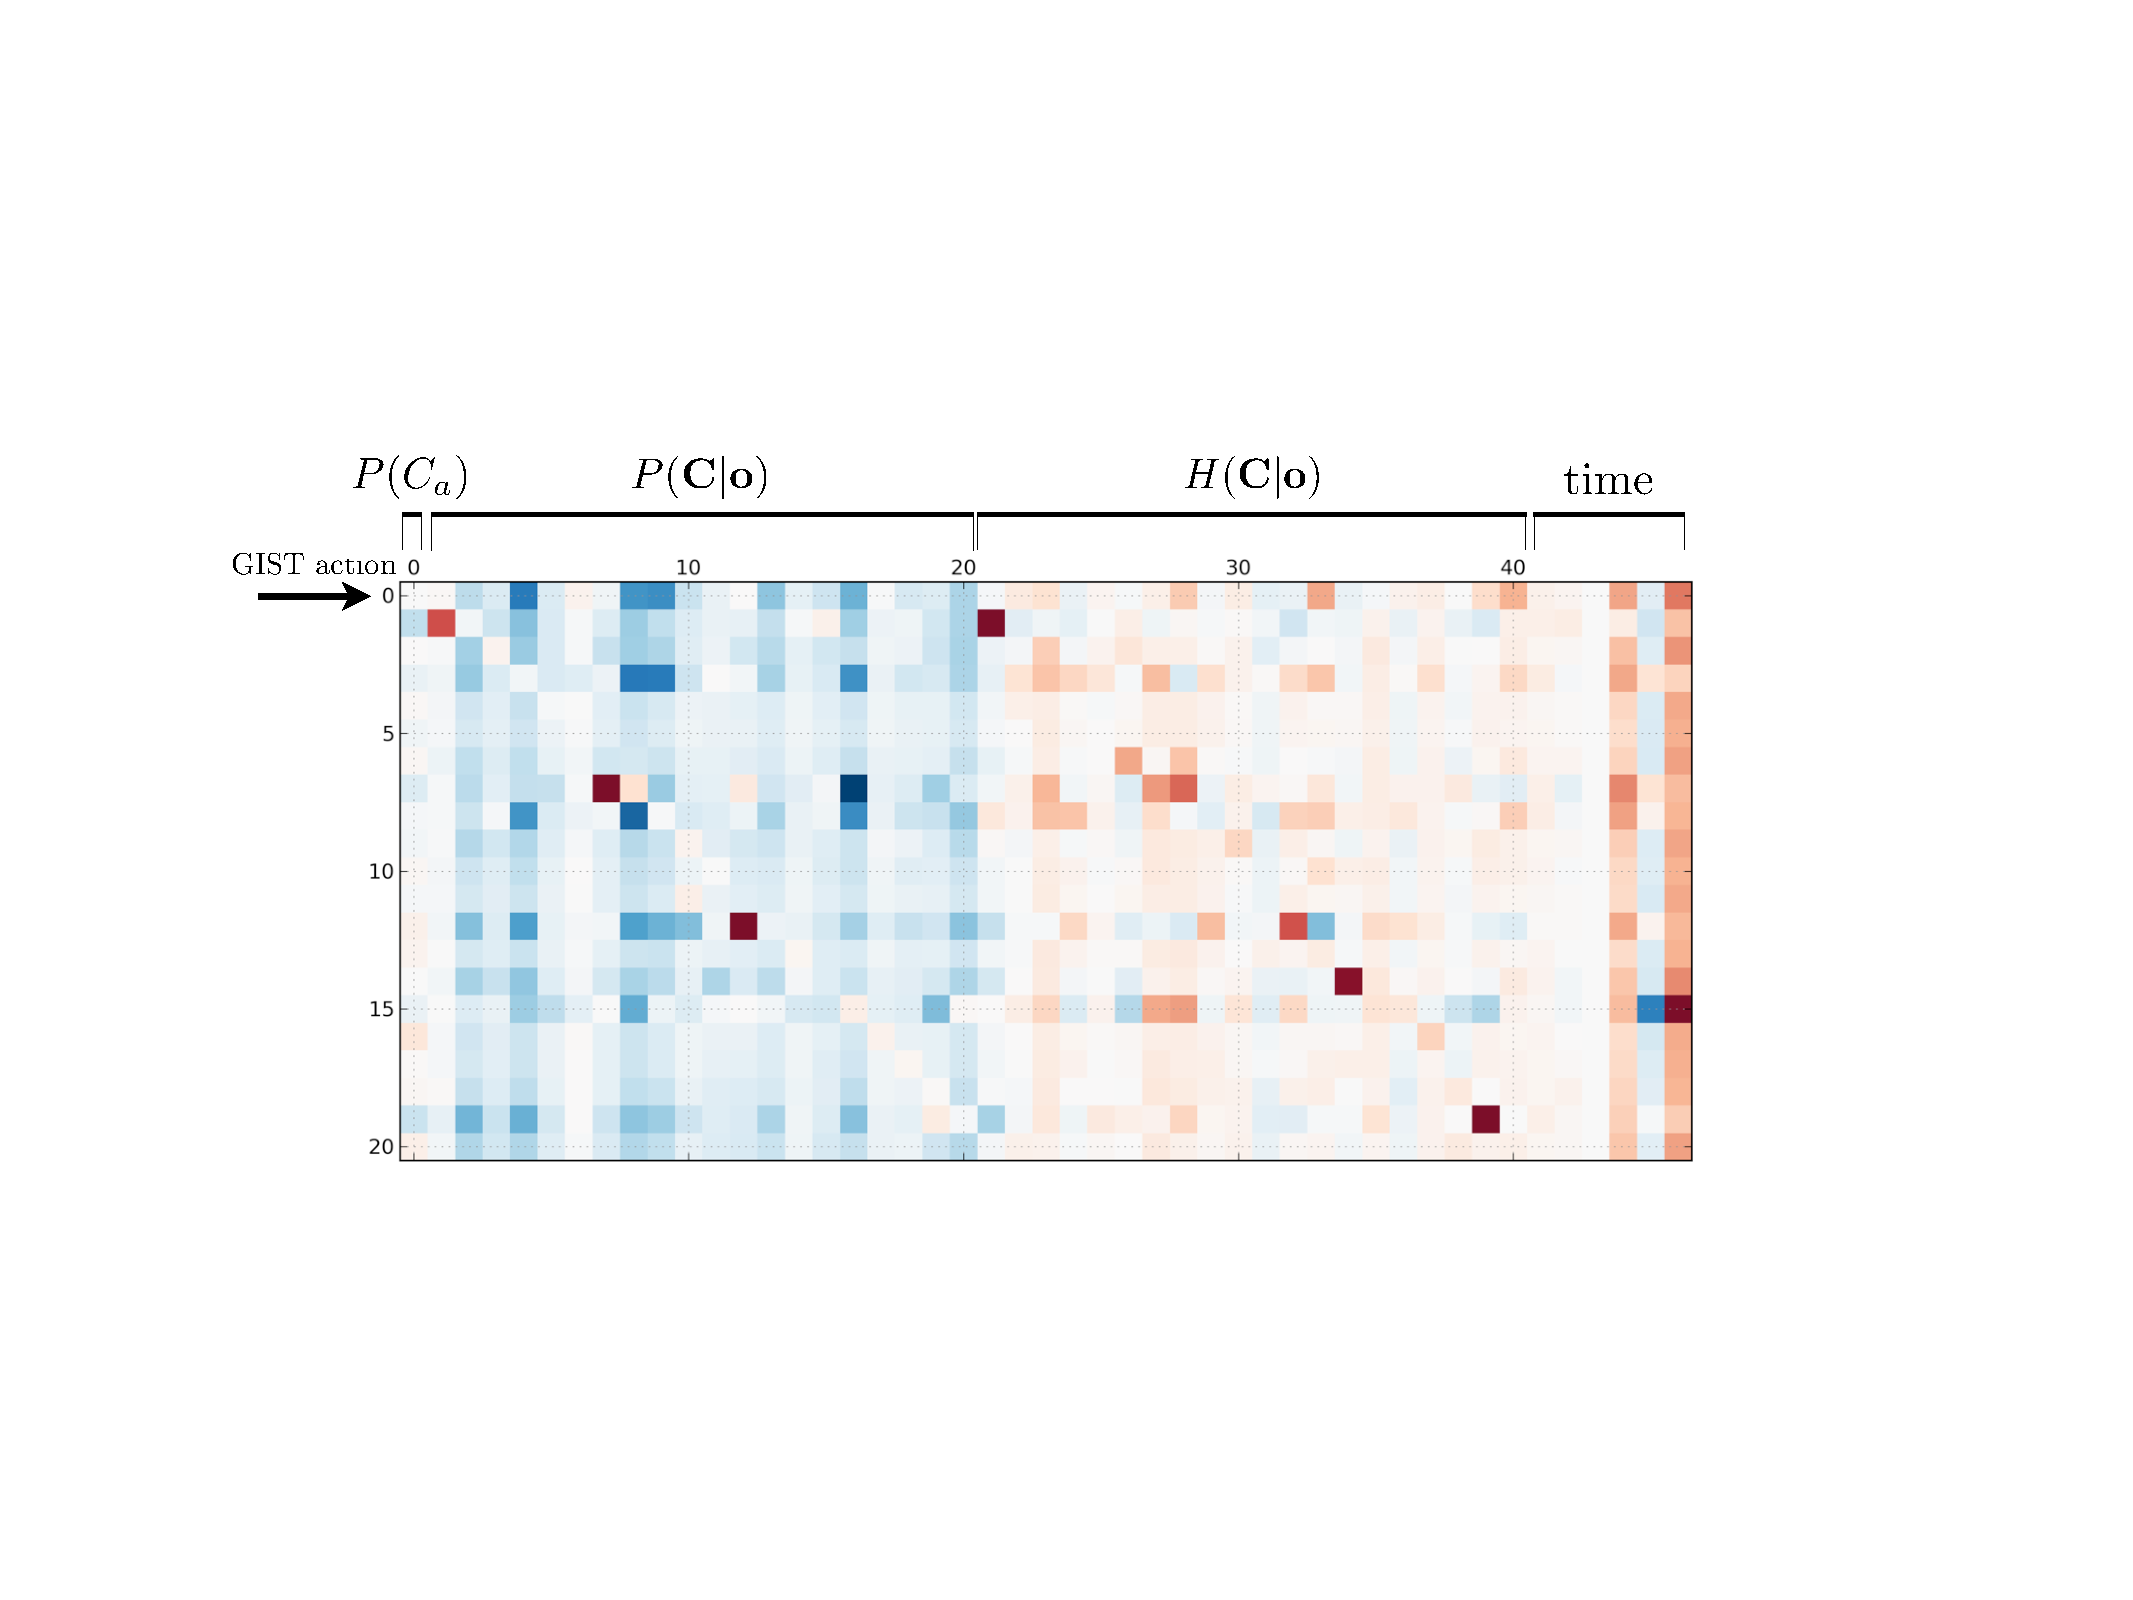
\includegraphics[width=\linewidth]{../../../2011-2012/figures/weights_rl}
    \caption{Reinforcement Learning}
\end{subfigure}
\caption[Learned policy weights for the detection approach.]{
Learned policy weights $\theta_\pi$ (best viewed in color: red corresponds to positive, blue to negative values).
The first row corresponds to the scene-level action, which does not generate detections itself but only helps reduce uncertainty about the contents of the image.
Note that in the greedy learning case, this action is learned to never be taken, but it is shown to be useful in the reinforcement learning case.
}
\label{fig:det_weights}
\end{figure}
